\documentclass[12pt]{article}
\usepackage{latexsym}
\usepackage{amssymb,amsmath}
\usepackage[pdftex]{graphicx}
\usepackage{color}
\usepackage{tikz}
\usepackage[margin=0.5in]{geometry}
\usepackage{epstopdf}

\begin{document}

\begin{center}
COMPUTER SCIENCE 20, SPRING 2014 \\
Module \#12 (Graph Coloring) \\
Author: Tawheed Abdul-Raheem
\end{center}

\begin{enumerate}

\item Find a four coloring for the graph below. Find a three coloring, or explain why no three coloring can exist. Find a two coloring, or explain why no two coloring can exist.

\begin{center}
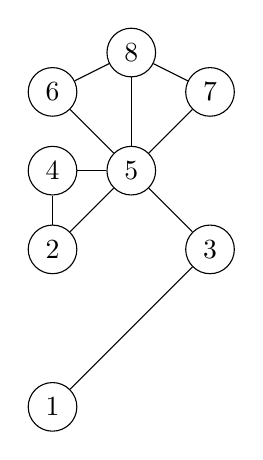
\begin{tikzpicture}
	\node (1) at (0,0) [shape=circle, draw] {1};
	\node (2) at (0,2) [shape=circle, draw] {2};
	\node (3) at (2,2) [shape=circle, draw] {3};
	\node (4) at (0,3) [shape=circle, draw] {4};
	\node (5) at (1,3) [shape=circle, draw] {5};
	\node (6) at (0,4) [shape=circle, draw] {6};
	\node (7) at (2,4) [shape=circle, draw] {7};
	\node (8) at (1,4.5) [shape=circle, draw] {8};


	\path 	[-]	(1) 	edge 	(3)
			(2)	edge	(4)
				edge 	(5)
			(3)	edge	(5)
			(4)	edge	(5)
			(5)	edge	(6)
				edge 	(7)
				edge 	(8)
			(6)	edge	(8)
			(7)	edge	(8);
\end{tikzpicture}
\end{center}

\textbf{Solution: } A two coloring would not be able to exist because we have a triangle in our graph.

\end{enumerate}
\end{document}
